\section{Related work}
\begin{figure*}[htbp]
  \centering
  % Requires \usepackage{graphicx}
  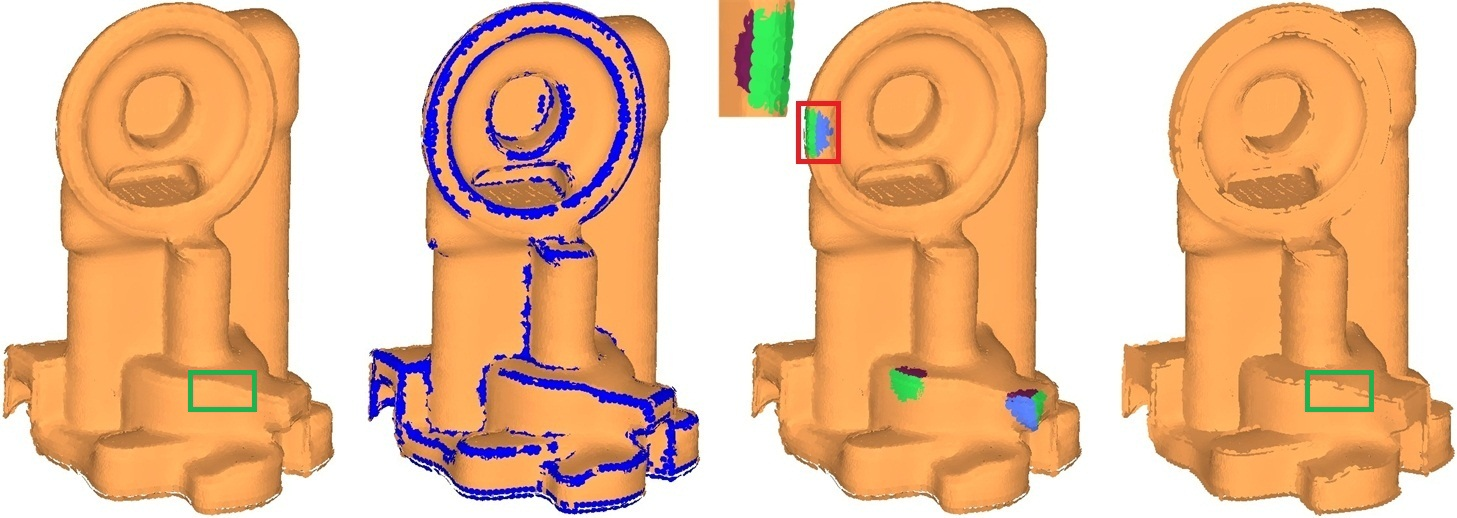
\includegraphics[width=1\linewidth]{oilpump_zj}\\
  \hspace{0 mm} (a) \hspace{38 mm} (b) \hspace{38 mm} (c)\hspace{38 mm} (d)
  \caption{Method overview.
         (a) The oil pump module with the normal computed by PCA. (b) Initial detected candidate feature points. (c) The classified subneighborhoods. The neighborhood within the red box contains three subneighborhoods rendered in blue, green and brown and the zoomed view is from left. (d) Estimated normals. Comparing (a) with (d), our method preserves the sharp features better, and the $RMS\_\tau$ introduced in section 5 is 0.6716 and 0.1308, respectively.} \label{fig:flow_chart}
\end{figure*}
%\subsection{Normal estimation}
Given a 3D point cloud, how to accurately estimate normals has been a primary concern in visual computing community. We briefly review it in this section.
%
We do not address the problem of normal orientation, which can be done separately \cite{CaoHLLS11, wang_vc12, seversky_smi11, LiuWang-SMI10, Huang-TOG09}.

%%%%%%%%%%%%%%%%%%%%%%%%%%%%%%%%%%%%%%%%%%%%%%%%%%%%%%%%%%%%%%%%%%%%%%%%%%%%%%%%%%%%%%%%%%%%%%%%%%%%%%%%%%%%
%%%%%%%%%%%%%%%%%%%%%%%%%%%%%%%%%%%%%%%%%%%%%%%%%%%%%%%%%%%%%%%%%%%%%%%%%%%%%%%%%%%%%%%%%%%%%%%%%%%%%%%%%%%%

The classical normal estimation method, proposed by Hoppe \etal \cite{DBLP:conf/siggraph/HoppeDDMS92} (PCA), defines the normal of a point as the eigenvector corresponding to the smallest eigenvalue of the covariance matrix of its neighbors.
They assume that the local neighborhood of any input point can be approximated by a plane.
%For each point , a least squares local plane is fitted to its k nearest neighbors by PCA. The normal of p is the eigenvector corresponding to the smallest eigenvalue of the covariance matrix.
%
There are a number of variants of this method which are compared carefully in~\cite{Klasing09}.
%
Guennebaud \etal \cite{GuennebaudG07} and Cazals \etal \cite{CazalsP03} used spheres and quadrics to replace planes, respectively.
%Other surfaces have been used too, e.g., spheres [GG07] or jets (a truncated Taylor expansion of a surface expression) such as quadrics [CP03].
%
Pauly \etal \cite{PaulyKKG03} proposed a weighted version of this basic approach by assigning Gaussian weights to its neighbors.
%By assigning Gaussian weights to p��s neighbors, a weighted version of this basic approach was proposed in [7,16].
%
By analysing the local noise, curvature and sample density, a method \cite{MitraN03} that adaptively chooses the size of neighborhood is proposed.
%For noisy point clouds, Mitra et al. [9] suggested an adaptive neighborhood size based on local properties, e.g.noisescale,curvature and sampling density.
%
Yoon \etal \cite{YoonLLIS07} took the ensemble technique from statistics to improve the robustness of PCA.
%Recently, the ensemble technique from statistics was used to improve the robustness of Hoppe et al.��s method such that noise and outliers can be well handled [17].
%
%The gradient of a local fitted algebraic sphere is used to compute a robust normal \cite{GuennebaudG07}.
%Guennebaud etal. [18] took the gradient of an algebraic sphere, which was fitted to the local neighborhood of p, to estimate the normal.
%
%Huang et al. [19] presented an interesting work on consolidating raw point clouds,in which weighted locally optimal projection (WLOP) is used to generate denoised, outlier-free and evenly distributed particles.The na sophisticated approach is employed to get reliable orientations for the normals computed by weighted PCA.
%
However, PCA and its variants tend to smooth sharp features since they actually are low-pass filters and usually need a large neighborhood to deal with noise.
%However, PCA and its variants are actually low-pass filters,thus any sharp features are necessarily smoothed out. However, all regression-based techniques tend to smooth sharp features, and thus fail to correctly estimate normals near edges (see Figure 1). The estimation quality also depends a lot on the size of the neighborhood used for regression: larger neighborhoods are needed to deal with noise, but they make sharp features even smoother.

%%%%%%%%%%%%%%%%%%%%%%%%%%%%%%%%%%%%%%%%%%%%%%%%%%%%%%%%%%%%%%%%%%%%%%%%%%%%%%%%%%%%%%%%%%%%%%%%%%%%%%%%%%%%
%%%%%%%%%%%%%%%%%%%%%%%%%%%%%%%%%%%%%%%%%%%%%%%%%%%%%%%%%%%%%%%%%%%%%%%%%%%%%%%%%%%%%%%%%%%%%%%%%%%%%%%%%%%%

Another class of methods is based on the improvement of preliminary normal estimation.
%Another class of methods is based on a preliminary normal estimation, which is improved.
%
The adaptive moving least squares method \cite{AlexaBCFLS01} and the robust local kernel regression method  \cite{DBLP:journals/cgf/OtireliGG09} estimate normals as the gradient of an implicit surface fitting the local points and their prescribed normals.
%Algorithms such as Moving Least Squares (MLS) [ABCO01], adaptive versions [PKKG03], or robust Local Kernel Regression (LKR) [?GG09] compute an implicit surface and estimate normals as the gradient of the surface.
%
Bilateral filtering proposed by \cite{DBLP:journals/cga/JonesDZ04} takes advantage of the difference between preliminary normals to recover sharp features.
%
Though those methods can obtain nearly correct normals for the points close to sharp features, their quality heavily relies on the input normals.
%They can retrieve sharp features, but they depend on a reliable prior estimation of input normals. Bilateral filtering [JDZ04] also preserves sharp features while smoothing even regions, but it can be slow and the quality relies on that of input normals too.
%This kind of method scan recover nearly correct normals for points near/on sharp features. However, as post-processing methods, all of them need good initial normals which at least roughly contain the sharp features. Moreover, iterative refining and many non-trivial parameters which need to be tuned carefully make these approaches quite tedious in actual applications.

%%%%%%%%%%%%%%%%%%%%%%%%%%%%%%%%%%%%%%%%%%%%%%%%%%%%%%%%%%%%%%%%%%%%%%%%%%%%%%%%%%%%%%%%%%%%%%%%%%%%%%%%%%%%
%%%%%%%%%%%%%%%%%%%%%%%%%%%%%%%%%%%%%%%%%%%%%%%%%%%%%%%%%%%%%%%%%%%%%%%%%%%%%%%%%%%%%%%%%%%%%%%%%%%%%%%%%%%%

Amenta \etal \cite{AmentaB99} first introduced the Delaunay/Voronoi technique into normal estimation.  They used the Voronoi diagram and the furthest vertex of the Voronoi cell to approximate the normals of noise-free point clouds.
%Delaunay/Voronoi based approaches for noise-free point-clouds regard the line through p and the furthest Voronoi vertex in p��s Voronoi cell,named pole, as the approximation of the normal for p [20].
%Dey��s method [DG06] relies on the construction of a Vorono? diagram and the search of the furthest vertex of the Vorono? cell.
%
By finding big Delaunay balls, Dey \etal \cite{DeyG06} applied this idea to noisy point-clouds.
%Deyetal. [21] extended the idea of pole to noisy point-clouds by finding big Delaunay balls.
%
%Also based on the Voronoi diagram, OuYang etal. [22] constructed a local Voronoi mesh for the neighbors of p and then fitted a group of quadric curves through which the directional tangent vectors could be obtained.
%
The combination of principal component analysis and Voronoi is proposed by Alliez \etal \cite{AlliezCTD07} to obtain more stable normals.
%Alliez et al. [ACSTD07] address this issue with a Vorono?-PCA method that provides some control over smoothness.
%Alliez etal. [23] presented an interesting combination of PCA and Voronoi based methods: Thus this method benefits from the local nature of PCA and the global partition quality of Voronoi based approach and more stable normals can be obtained.
%
However, none of them can estimate the normals of points near/on sharp features accurately.
%However, the sharp features in point-clouds are not considered either. %nearby

%%%%%%%%%%%%%%%%%%%%%%%%%%%%%%%%%%%%%%%%%%%%%%%%%%%%%%%%%%%%%%%%%%%%%%%%%%%%%%%%%%%%%%%%%%%%%%%%%%%%%%%%%
%%%%%%%%%%%%%%%%%%%%%%%%%%%%%%%%%%%%%%%%%%%%%%%%%%%%%%%%%%%%%%%%%%%%%%%%%%%%%%%%%%%%%%%%%%%%%%%%%%%%%%%%%

%More recently, both noise and sharp features have been treated explicitly by Li et al. [LSK10], combining a robust local noise estimation and a RANSAC-like method that is parameterized by the estimated noise scale. It handles well noise and outliers. But it is not very fast (typically around half an hour for 1.5 million points). Besides, it does not address variation of density at edges.
%The key ingredients of our approach are a robust noise-scale estimator and a kernel density estimation (KDE) based objective function
More recently, by combining a robust noise-scale estimator and a kernel density estimation, Li \etal \cite{DBLP:journals/cg/LiSKCDJ10} (RNE) proposed a robust normal estimation method which can handle noise and sharp features well. However, it does not address variation of density at edges, for the kernel density estimation favors the sides with high density. Boulch \etal \cite{DBLP:journals/cgf/BoulchM12} (HF) used a stop criterion inherited from robust statistics to speed the Randomized Hough Transform and a uniform sampling strategy to overcome the density anisotropy. However, when the dihedral angle between the two planes forming the sharp feature is large, the difference is small between normals produced by triples sampled from different sides, so these normals are likely to vote for the same bin. Consequently, it tends to generate smooth effect near sharp features.

%%%%%%%%%%%%%%%%%%%%%%%%%%%%%%%%%%%%%%%%%%%%%%%%%%%%%%%%%%%%%%%%%%%%%%%%%%%%%%%%%%%%%%%%%%%%%%%%%%%%%%%%
%%%%%%%%%%%%%%%%%%%%%%%%%%%%%%%%%%%%%%%%%%%%%%%%%%%%%%%%%%%%%%%%%%%%%%%%%%%%%%%%%%%%%%%%%%%%%%%%%%%%%%%%
%\subsection{Subspace Clustering}
%Subspace clustering aims to cluster the high dimensional data sets into multiple low-dimensional linear subspaces simultaneously and has been widely used in computer vision, image processing, and data regression, etc. (see [PHL04, Vid10] and references therein). We treat the segmentation of a neighbourhood as a subspace clustering problem .
